\documentclass[a4paper, 12pt]{article}

% Добавляем новые пакеты
\usepackage[english, russian]{babel}    % Пакет для поддержки русского языка
\usepackage[T1, T2A]{fontenc}           % Загружаем пакет с поддержкой кирилицы
\usepackage[utf8]{inputenc}             % Загружаем пакет с поддержкой кодировки файла и символов
\usepackage{ragged2e}                   % Загружаем пакет для выравнивания текста
\usepackage{graphicx}                   % Загружаем пакет для добавления различной графики (pdf, jpg, png)
\usepackage{import}                     % Загружаем пакет для продвинутого импорта, в частности изображений pdf_tex из графического редактора inkscape (\import{<path to file>}{<filename>.pdf_tex})
\usepackage{subcaption}                 % Пакет для поддержки сетки из фигур, например в две колонки или матрицей
\usepackage{float}                      % Пакет для улучшенного размещения изображенией (ниже используется опция H в команде \begin{figure}[H])
\usepackage{geometry}                   % Пакет для управления отступами на странице (см. далее вызываем \geometry)
\usepackage{amsmath}                    % Добавляем крутую поддержку математики, в частности /align
\usepackage{amsfonts}                   % Пкет с мтематическими шрифтами вроде \mathbb и др.
\usepackage{tabu}                       % Пакет с прокаченными таблицами
\usepackage{booktabs}                   % Крутые вертикальные разделители
\usepackage[dvipsnames]{xcolor}         % Рассширенная поддержка цветов
\usepackage[colorlinks]{hyperref}
\usepackage{indentfirst}                % Пакет, чтобы починить красную строку
\usepackage{listings}                   % Поддержка листингов, оформления кода программы
\usepackage{src/vpdtitle}               % Титульный лист (смотри файл vpdtitle.sty)

\usepackage{titletoc}
\dottedcontents{section}[2.3em]{}{2.3em}{6pt}
\dottedcontents{subsection}[2.3em]{}{2.3em}{6pt}
\dottedcontents{subsubsection}[2.3em]{}{2.3em}{6pt}

% Устанавливает отступы на странице
\geometry{left=2cm, right=2cm, bottom=2cm, top=2cm}

% Настараиваем красивые цвета для ссылок на формулы, фигуры (изображения) и другие элементы.
\hypersetup{
    linkcolor=blue,
    filecolor=magenta,
    urlcolor=cyan
}

% Настраиваем супер красивые листинги с попомщью пакетов listings и xcolor
\definecolor{codegreen}{rgb}{0,0.6,0}
\definecolor{codegray}{rgb}{0.5,0.5,0.5}
\definecolor{codepurple}{rgb}{0.58,0,0.82}
\definecolor{backcolour}{rgb}{0.95,0.95,0.92}

\lstdefinestyle{codestyle}{
    backgroundcolor=\color{backcolour},
    commentstyle=\color{codegreen},
    keywordstyle=\color{magenta},
    numberstyle=\tiny\color{codegray},
    stringstyle=\color{codepurple},
    basicstyle=\ttfamily\footnotesize,
    breakatwhitespace=false,
    breaklines=true,
    captionpos=b,
    keepspaces=true,
    numbers=left,
    numbersep=5pt,
    showspaces=false,
    showstringspaces=false,
    showtabs=false,
    tabsize=2
}

\lstset{style=codestyle}
\lstset{extendedchars=\true}

%%%%%%%%%%%%%%%%%%%%%%%%%%%%%%%%%%%%%%%%%%%%%%%%
%% Заполнение титульного листа
%%%%%%%%%%%%%%%%%%%%%%%%%%%%%%%%%%%%%%%%%%%%%%%%
\title{
Модели линейных динамических систем
}

% Тут укажите автора
\author{Иван М. Бакланов}
\affil{465112, ibaklanov@niuitmo.ru}

\author{Владимир В. Ананичев}
\affil{464994, vandmitrievic@mail.ru}
% Впишите данные о том, кто будет проверять работу
\author{Даниил А. Юлдашев}
\affil{468158}

\supervisor{Артем В. Пашенко}

% Краткое описание того, что сделали в работе
\abstract{
Ознакомление с основными представлениями и
принципами построения моделей линейных стационарных динамических систем.
}

% Подберите 3-5 ключевых слова, отличающих эту работу от всех остальных
\keywords{
    Simulink, Matlab, Linear systems, Control theory
}

\date{\today}







%%%%%%%%%%%%%%%%%%%%%%%%%%%%%%%%%%%%%%%%%%%%%%%%
% Начала всего-всего текста. Здесь идет сам документ, все пишется именно сюда
%%%%%%%%%%%%%%%%%%%%%%%%%%%%%%%%%%%%%%%%%%%%%%%%
\begin{document}

\maketitle

\tableofcontents

\newpage


\section{Задание №1}
\section{Построение схемы и вывод начальных условий}
Зададим следующую линейную систему с управлением.
\[
\dddot{y}(t) + 8\ddot{y}(t) + 19\dot{y}(t) + 12y(t) = 72\ddot{u}(t) + 36\dot{u}(t) + 42u(t)
\]
Построим схему в Simulink, которая моделирует данную систему.
\begin{figure}[H]
    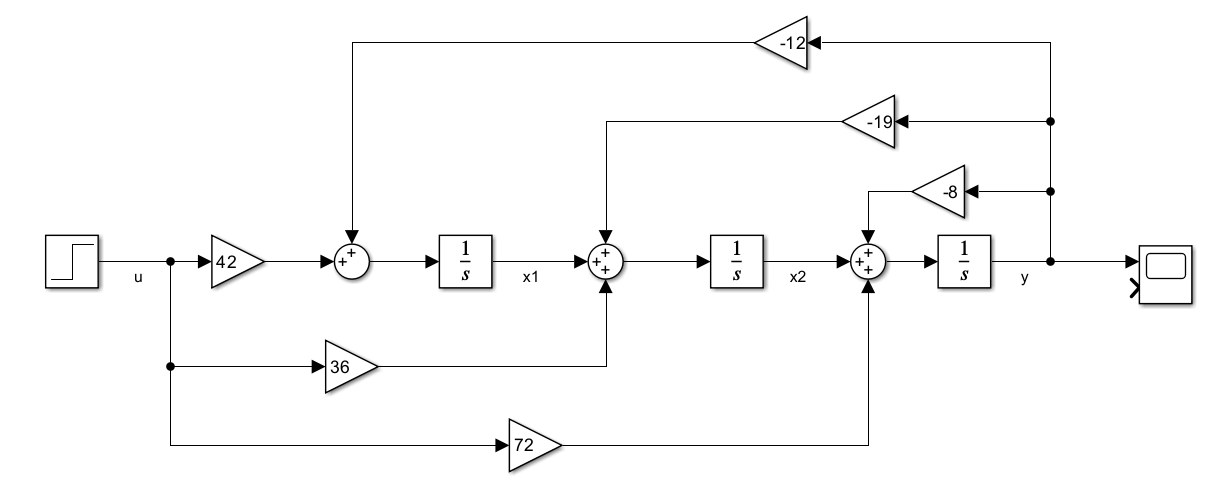
\includegraphics[width=\textwidth]{images/model1.jpg}
    \caption{Схема моделирования задания 1}
    \label{fig:1}
\end{figure}
Рассмотрим, как получена данная схема и как в ней должны задаваться начальные условия

\[
(p^3 + 8p^2 + 19p + 12)[y] = (72p^2 + 36p + 42)[u]
\]

\[
y = \frac{1}{p^3}((72p^2 + 36p + 42)[u] - (8p^2 + 19p + 12)[y])
\]
\[
y = \frac{1}{p}(72u - 8y + \frac{1}{p}(36u - 19y + \frac{1}{p}(42u - 12y)))
\]

Введём обозначения выходов интеграторов (справа налево):
\begin{itemize}
    \item $x_1$ --- выход внешнего (правого) интегратора
    \item $x_2$ --- выход среднего интегратора
    \item $x_3 = y$ --- выход самого внутреннего (леввого) интегратора
\end{itemize}

Тогда система дифференциальных уравнений принимает вид:
\[
    \dot{x}_1 = 42u - 12y
\]
\[
    \dot{x}_2 = 36u - 19y + x_1
\]
\[
    \dot{y} = 72u - 8y + x_2
\]

Из уравнения для $\dot{y}$:
\[
    x_2 = \dot{y} + 8y - 72u
\]

Из уравнения для $\dot{x}_2$:
\[
    x_1 = \dot{x}_2 - 36u + 19y
\]
\[
    x_1 = (\ddot{y} + 8\dot{y} - 72\dot{u}) - 36u + 19y
\]
\[
    x_1 = \ddot{y} + 8\dot{y} - 72\dot{u} - 36u + 19y
\]

Заданные начальные условия:
\[
    y(0) = 1, \quad \dot{y}(0) = 0.3, \quad \ddot{y}(0) = 0.7
\]


\[
    x_2(0) = \dot{y}(0) + 8y(0) - 72u(0) = 0.3 + 8\cdot 1 = 8.3
\]

\[
    x_1(0) = \ddot{y}(0) + 8\dot{y}(0) - 72\dot{u}(0) - 36u(0) + 19y(0)
\]
\[
    x_1(0) = 0.7 + 8\cdot 0.3  + 19\cdot 1
\]
\[
    x_1(0) = 0.7 + 2.4 + 19 = 22.1
\]

\[
    x_1(0) = 22.1
\]
\[
    x_2(0) = 8.3
\]
\[
    x_3(0) = 1.0
\]
Это и есть начальные условия для интеграторов в схеме.
\newpage

\subsection{Константный входной сигнал}
Подадим входной сигнал в виде функции \(1(t)\)
\begin{center}
    \begin{figure}[H]
        \includegraphics[width=0.8\textwidth]{images/ut1.jpg}
        \caption{Входной сигнал 1(t)}
        \label{fig:2}
    \end{figure}
\end{center}
Тогда получим выходной сигнал
\begin{center}
    \begin{figure}[H]
        \includegraphics[width=0.8\textwidth]{images/yt1.jpg}
        \caption{Выходной сигнал y(t)}
        \label{fig:3}
    \end{figure}
\end{center}
\subsection{Отсутствие входного сигнала}
Теперь подадим на вход \(u(t) = 0\) и установим начальные условия. Тогда на выходе мы получим следующий сигнал
\begin{center}
    \begin{figure}[H]
        \includegraphics[width=0.8\textwidth]{images/no0yt1.jpg}
        \caption{Выходной сигнал y(t) при u(t) = 0 и ненулевых начальных условиях}
        \label{fig:4}
    \end{figure}
\end{center}

\subsection{Константный входной сигнал при ненулевых начальных условиях}
Теперь оставим ненулевые начальные условия из предыдущего пункта и подадим на вход сигнал из первого пункта.

\begin{center}
    \begin{figure}[H]
        \includegraphics[width=0.8\textwidth]{images/no0ytwu1.jpg}
        \caption{Выходной сигнал y(t) при u(t) = 1(t) и ненулевых начальных условиях}
        \label{fig:5}
    \end{figure}
\end{center}

Теперь достроим на этом графике график функции \(f(t) = y_1(t) + y_2(t)\), где \(y_1(t)\) - это выход системы с ненулевыми начальными условиями и нулевым входом, а \(y_2(t)\) - это выход системы с нулевыми начальными условиями и константным входом.
\begin{center}
    \begin{figure}[H]
        \includegraphics[width=0.8\textwidth]{images/ft1.jpg}
        \caption{Сравнительный график \(f(t)\) и \(y(t)\)}
        \label{fig:6}
    \end{figure}
\end{center}

\subsection{Анализ}
Как мы можем судить по уравнениям, система физически реализуема, имеет относительный порядок 1.
\\

Полюса системы
\[
p_1 = -4 \quad p_2 = -3 \quad p_3 = -1
\]
Все они находятся в левой комплексной полуплоскости, значит, система ассимптотически устойчива.
Это видно из графиков, каждый из которых имеет горизонтальную ассимптоту. Также, судя по полюсам, система имеет апериодический характер свободного движения, что видно на Рис. 4.
\\

Нули системы
\[
p_{1,2} = -0.25 \pm 0.433i
\]
Нули системы комплексные, а значит управление добавляет к свободному движению колебательную составляющую.
Действительная часть нулей - отрицательная, следовательно колебания, вносимые управлением - затухающие.
\\

Влияние начальных условий можно увидеть на графиках, в виде смещения точки \((0, y(0))\).
\\

В последнем пункте задания видно, что сумма \(f(t)\) идентична выходу системы с начальными условиями и входом \(1(t)\).
Это вытекает из того, что \(f(t)\) есть сумма свободного движения(выход системы при нулевом входе и ненулевых начальных условиях)
и влияния управления на систему(выход системы с управлением вида \(1(t)\) и нулевыми начальными условиями).

\newpage
\section{Задание №2}

Запишем передаточную функцию для системы из предыдущего задания
\[
W(p) = \frac{72p^2 + 36p + 42}{p^3 + 8p^2 + 19p +12}
\]

\subsection{Каноническая управляемая форма}
Матрицы для канонической управляемой формы
\[
A = \begin{bmatrix}
    0&1&0\\
    0&0&1\\
    -12&-19&-8\\
\end{bmatrix} \quad B = 
\begin{bmatrix}
    0\\0\\1    
\end{bmatrix}
\]
\[
C = \begin{bmatrix}
    42&36&72
\end{bmatrix} \quad D=\begin{bmatrix}
    0
\end{bmatrix}
\]
запишем в виде системы
\[
\begin{cases}
    \dot{x_1} = x_2\\
    \dot{x_2} = x_3\\
    \dot{x_3} = -12x_1 - 19x_2 - 8x_3 + u\\
    y = 42x_1 + 36x_2 + 72x_3
\end{cases}
\]

Для определения начального состояния воспользуемся соотношением

\[
y^{(i)}(0) = CA^i x(0),
\]

принимая начальное значение управляющего воздействия равным нулю:
\(u(0)=0\).

Для $i=0$ получаем условие на выход:

\[
y(0) = Cx(0)
=
\begin{bmatrix}
42 & 36 & 72
\end{bmatrix}
\begin{bmatrix}
x_1(0)\\
x_2(0)\\
x_3(0)
\end{bmatrix}.
\]

Следовательно,

\[
y(0) =
42x_1(0) + 36x_2(0) + 72x_3(0).
\]

Для $i=1$ вычислим произведение $CA$:

\[
CA =
\begin{bmatrix}
42 & 36 & 72
\end{bmatrix}
\begin{bmatrix}
0 & 1 & 0\\
0 & 0 & 1\\
-12 & -19 & -8
\end{bmatrix}
=
\begin{bmatrix}
-864 & -1326 & -540
\end{bmatrix}.
\]

Следовательно,

\[
\dot{y}(0) =
-864x_1(0) - 1326x_2(0) - 540x_3(0).
\]

Для $i=2$ сначала вычислим матрицу $A^2$:

\[
A^2 =
\begin{bmatrix}
0 & 0 & 1\\
-12 & -19 & -8\\
96 & 140 & 45
\end{bmatrix}.
\]

Тогда

\[
CA^2 =
\begin{bmatrix}
42 & 36 & 72
\end{bmatrix}
\begin{bmatrix}
0 & 0 & 1\\
-12 & -19 & -8\\
96 & 140 & 45
\end{bmatrix}
=
\begin{bmatrix}
6480 & 9396 & 2994
\end{bmatrix}.
\]

Следовательно,

\[
\ddot{y}(0) =
6480x_1(0) + 9396x_2(0) + 2994x_3(0).
\]

Таким образом, для определения начального состояния необходимо решить
систему

\[
\begin{cases}
42x_1(0) + 36x_2(0) + 72x_3(0) = y(0),\\
-864x_1(0) - 1326x_2(0) - 540x_3(0) = \dot{y}(0),\\
6480x_1(0) + 9396x_2(0) + 2994x_3(0) = \ddot{y}(0).
\end{cases}
\]

Подставляя заданные начальные условия

\[
y(0)=1,\qquad
\dot{y}(0)=0.7,\qquad
\ddot{y}(0)=0.3,
\]

получаем систему

\[
\begin{cases}
42x_1 + 36x_2 + 72x_3 = 1,\\
-864x_1 - 1326x_2 - 540x_3 = 0.7,\\
6480x_1 + 9396x_2 + 2994x_3 = 0.3.
\end{cases}
\]

Решение данной системы:

\[
\begin{aligned}
x_1(0) &\approx 0.032,\\
x_2(0) &\approx -0.024,\\
x_3(0) &\approx 0.007.
\end{aligned}
\]


Промоделируем данную систему

\begin{figure}[H]
    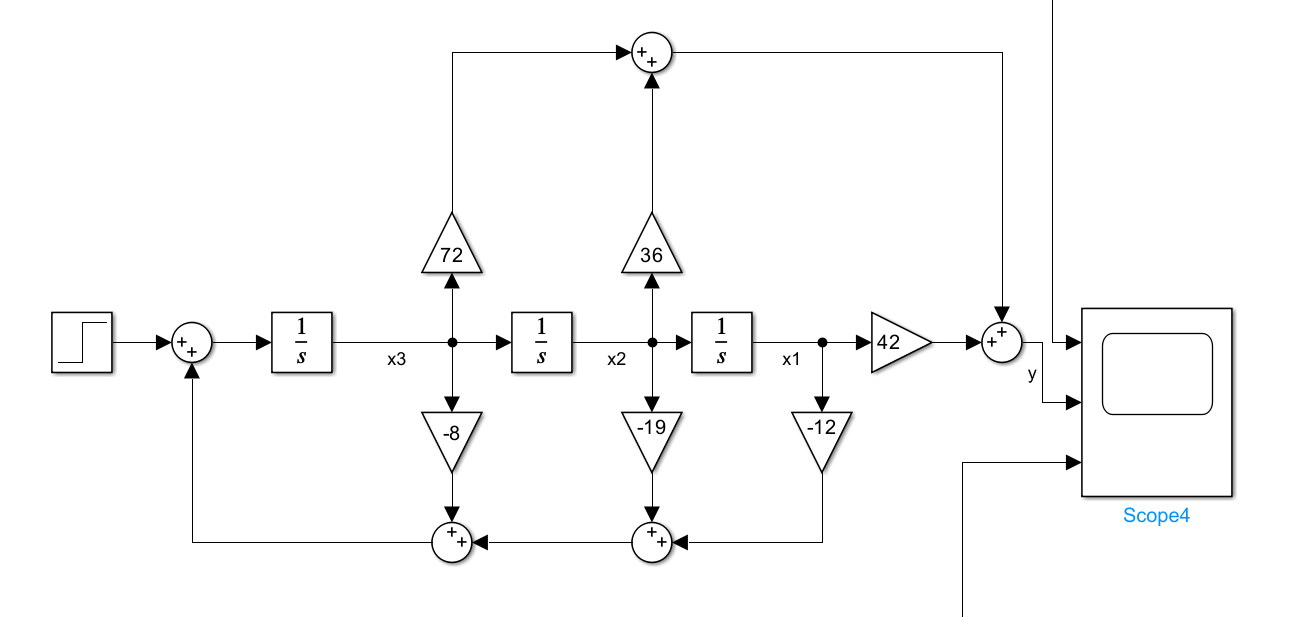
\includegraphics[width=\textwidth]{images/model2con.jpg}
    \caption{Схема моделирования системы в канонической управляемой форме}
    \label{fig:1}
\end{figure}

На выходе системы получаем следующий сигнал.

\begin{figure}[H]
    \includegraphics[width=0.8\textwidth]{images/conyt2.jpg}
    \caption{Выходной сигнал системы в канонической управляемой форме}
    \label{fig:1}
\end{figure}

\subsection{Каноническая диагональная форма}

Для реализации полученной передаточной функции в канонической диагональной
форме используем разложение

\[
W(p) =
\frac{72p^2 + 36p + 42}{(p+4)(p+3)(p+1)}
=
\frac{350}{p+4}
-\frac{291}{p+3}
+\frac{13}{p+1}.
\]

В соответствии с полученным разложением структурная схема имеет вид

\[
A =
\begin{bmatrix}
-4 & 0 & 0\\
0 & -3 & 0\\
0 & 0 & -1
\end{bmatrix},
\qquad
B =
\begin{bmatrix}
350\\
-291\\
13
\end{bmatrix},
\]

\[
C =
\begin{bmatrix}
1 & 1 & 1
\end{bmatrix},
\qquad
D =
\begin{bmatrix}
0
\end{bmatrix}.
\]

Аналогично предыдущему пункту найдём начальные условия для системы.

Для $i=0$ получаем условие на выход:

\[
y(0)=Cx(0)
=
\begin{bmatrix}
1 & 1 & 1
\end{bmatrix}
\begin{bmatrix}
x_1(0)\\
x_2(0)\\
x_3(0)
\end{bmatrix},
\]

откуда

\[
y(0)=x_1+x_2+x_3.
\]

Для $i=1$:

\[
CA =
\begin{bmatrix}
1 & 1 & 1
\end{bmatrix}
\begin{bmatrix}
-4 & 0 & 0\\
0 & -3 & 0\\
0 & 0 & -1
\end{bmatrix}
=
\begin{bmatrix}
-4 & -3 & -1
\end{bmatrix}.
\]

Следовательно,

\[
\dot{y}(0)
=
-4x_1-3x_2-x_3.
\]

Для $i=2$ сначала вычислим

\[
A^2 =
\begin{bmatrix}
16 & 0 & 0\\
0 & 9 & 0\\
0 & 0 & 1
\end{bmatrix}.
\]

Тогда

\[
CA^2 =
\begin{bmatrix}
1 & 1 & 1
\end{bmatrix}
\begin{bmatrix}
16 & 0 & 0\\
0 & 9 & 0\\
0 & 0 & 1
\end{bmatrix}
=
\begin{bmatrix}
16 & 9 & 1
\end{bmatrix}.
\]

Следовательно,

\[
\ddot{y}(0)
=
16x_1+9x_2+x_3.
\]

Подставляя заданные начальные условия

\[
y(0)=1,\qquad
\dot{y}(0)=0.7,\qquad
\ddot{y}(0)=0.3,
\]

получаем систему уравнений

\[
\begin{cases}
x_1+x_2+x_3=1,\\
-4x_1-3x_2-x_3=0.7,\\
16x_1+9x_2+x_3=0.3.
\end{cases}
\]

Решение данной системы имеет вид

\[
\begin{aligned}
x_1(0) \approx 2.033 \\
x_2(0) = -3.9 \\
x_3(0) \approx 2.867.
\end{aligned}
\]

Смоделируем данную систему.

\begin{center}
    \begin{figure}[H]
        \includegraphics[width=0.8\textwidth]{images/model2diag.jpg}
        \caption{Модель системы в канонической диагональной форме}
        \label{fig:6}
    \end{figure}
\end{center}

Выходной сигнал.

\begin{center}
    \begin{figure}[H]
        \includegraphics[width=0.8\textwidth]{images/diagyt2.jpg}
        \caption{Выход системы в канонической диагональной форме}
        \label{fig:6}
    \end{figure}
\end{center}

Теперь построим на одном графике выход всех трёх форм системы.

\begin{center}
    \begin{figure}[H]
        \includegraphics[width=0.8\textwidth]{images/compare.jpg}
        \caption{Сравнение выходов различных форм системы}
        \label{fig:6}
    \end{figure}
\end{center}

Таким образом при помощи моделирования показано, что разницы в выходе различных представлений систем нет.
\newpage

\section{Задание №3}
Запишем условие задания в виде матриц A и B для многоканальной системы.
\[
A(p) = \begin{bmatrix}
    p+16&p+2\\
    p+5&p+7
\end{bmatrix}
B(p) = \begin{bmatrix}
    7&7\\
    5&6
\end{bmatrix}
\]
Найдём матрицу передаточных функций.
\[
W(p) = A(p)^{-1}B(p) = 
\frac{1}{16p+102}\begin{bmatrix}
    p+7&-(p+5)\\
    -(p+2)&p+16
\end{bmatrix}\begin{bmatrix}
    7&7\\
    5&6
\end{bmatrix}=
\]
\[
=\frac{1}{16p+102}\begin{bmatrix}
    2p+39&p+37\\
    -2p+45&-p+61
\end{bmatrix}
\]

Составим схему моделирования системы в форме вход-выход.

\begin{center}
    \begin{figure}[H]
        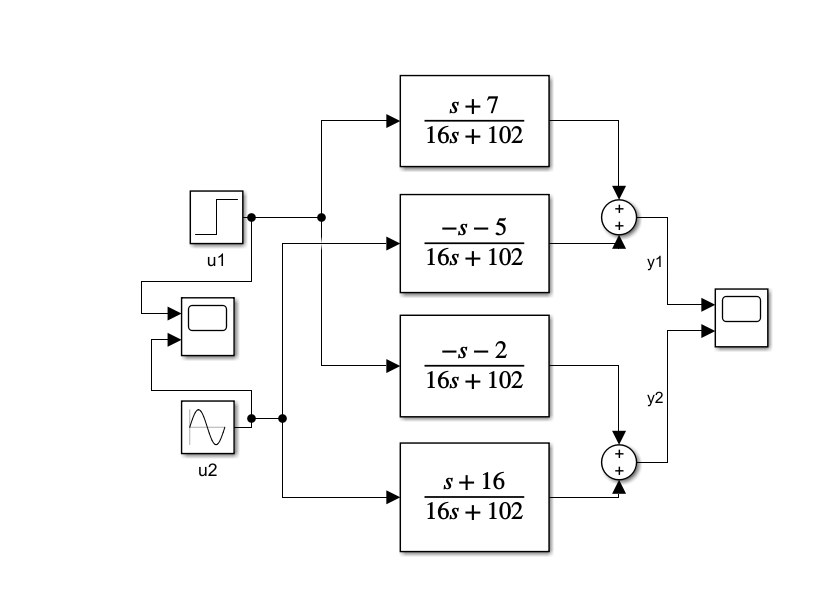
\includegraphics[width=0.8\textwidth]{images/model3.jpg}
        \caption{Модель многоканальной системы в виде ВВ}
        \label{fig:6}
    \end{figure}
\end{center}

Подадим на входы следующие сигналы. 

\begin{center}
    \begin{figure}[H]
        \includegraphics[width=0.8\textwidth]{images/t3in.jpg}
        \caption{Вход системы в виде ВВ}
        \label{fig:6}
    \end{figure}
\end{center}

Получим следующие выходы

\begin{center}
    \begin{figure}[H]
        \includegraphics[width=0.8\textwidth]{images/t3out.jpg}
        \caption{Выходы многоканальной системы}
        \label{fig:6}
    \end{figure}
\end{center}

\newpage
\section{Задание №4}
Рассмотрим многоканальную динамическую систему в форме вход-состояние-выход, заданную матрицами.
\[
A = \begin{bmatrix}
    0&-4\\
    1&-5
\end{bmatrix}
\quad
B = \begin{bmatrix}
    1&4\\
    6&7
\end{bmatrix}
\]
\[
C = \begin{bmatrix}
    8&5\\
    1&8
\end{bmatrix}
\quad
D = [0]
\]
Тогла в форме системы уравнений она примет вид.
\[
\begin{cases}
    \dot{x_1} = -4x_2 + u_1 + 4u_2\\
    \dot{x_2} = x_1 - 5x_2 + 6u_1 + 7u_2\\
    y_1 = 8x_1 + 5x_2\\
    y_2 = x_1 + 8x_2
\end{cases}
\]
Составим схему моделирования этой системы.
\begin{center}
    \begin{figure}[H]
        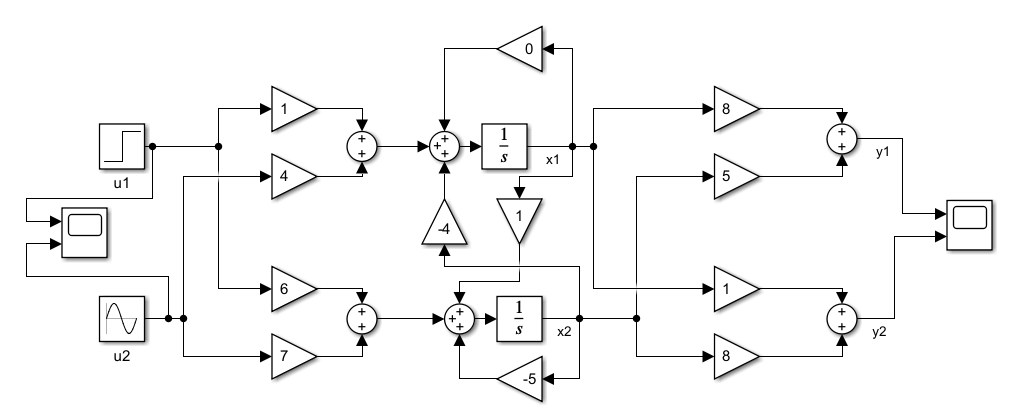
\includegraphics[width=0.8\textwidth]{images/model4.jpg}
        \caption{Модель многоканальной системы в виде ВСВ}
        \label{fig:6}
    \end{figure}
\end{center}
Подадим на вход такие же сигналы, что и в предыдущем задании 
\begin{center}
    \begin{figure}[H]
        \includegraphics[width=0.8\textwidth]{images/t4.jpg}
        \caption{Выходы многоканальной системы ВСВ}
        \label{fig:6}
    \end{figure}
\end{center}
\newpage
\section{Выводы}
В ходе выполнения лабораторной работы были изучены основные представления и принципы построения математических моделей линейных стационарных динамических систем, а также закреплены навыки их имитационного моделирования в среде MATLAB/Simulink. 

Была исследована одноканальная система в форме «вход-выход», для которой рассчитаны начальные условия вспомогательной переменной и экспериментально подтвержден принцип суперпозиции: полный отклик системы действительно равен сумме свободного и вынужденного движений. Далее эта же система была преобразована в форму «вход-состояние-выход» в канонической управляемой и канонической диагональной формах. С помощью матричного метода $y^{(i)}(0) = CA^i x(0)$ были корректно найдены начальные условия для переменных состояния, а последующее компьютерное моделирование наглядно доказало полную эквивалентность всех трех представлений, так как их выходные сигналы полностью совпали на сравнительном графике.

Также в работе были рассмотрены многоканальные динамические системы. Для них была найдена передаточная матрица в форме «вход-выход» и построена соответствующая схема моделирования, после чего система была описана через матрицы состояния, управления, наблюдения и связи в форме «вход-состояние-выход». Таким образом, работа позволила получить практический опыт аналитического перехода между различными формами описания линейных систем и убедиться в том, что выбор базиса пространства состояний или вида математической модели не влияет на физические свойства и итоговые динамические характеристики объекта управления.
\end{document}

